\documentclass{beamer}
\usepackage{graphicx}
\usepackage{listingsutf8}
\lstset{basicstyle=\ttfamily,breaklines=true}
\graphicspath{ {../images/} }
\usetheme{metropolis}

\begin{document}

\title{Analyse de couverture urbaine par homologie persistante : cas du 
    développement des transports publics}
\author{Elowan ; 10381}
\date{\today}

\maketitle

\begin{frame}
    \frametitle{Le but}    
    \textbf{Trouver les zones les moins biens desservies par un réseau de métros.}
    
    En convertissant des données géographiques en représentation géométrique
    puis en effectuant une analyse topologique de l'espace représenté.

    \begin{figure}
        % 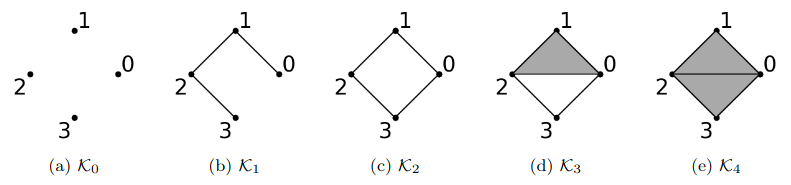
\includegraphics[width=\textwidth]{filtration}
        \centering
        \caption{Carte vers représentation géoQ vers cartes avec triangles}
    \end{figure}
    
    
\end{frame}

\begin{frame}
    \frametitle{Plus en détail : l'homologie persistante}
    \begin{figure}
        % 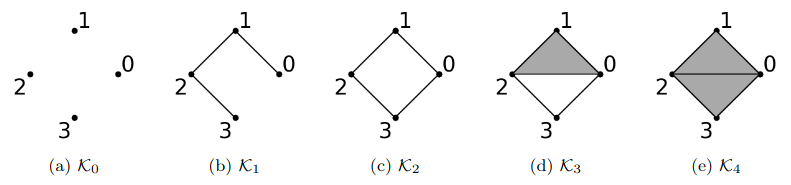
\includegraphics[width=\textwidth]{filtration}
        \centering
        \caption{Tore discrétisé, avec un zoom sur une partie du tore}
    \end{figure}
\end{frame}

\begin{frame}
    \frametitle{Définitions}
    \begin{block}{Simplexe}
        Généralisation du triangle en dimension $n$, c'est l'objet le plus simple 
        que l'on puisse construire qui ait $n$ dimension
    \end{block}

    \begin{block}{Face}
        La face de $\sigma$ un simplexe de dimension $n$ est un simplexe $\sigma'$
        de dimension $n-1$ constituant $\sigma$.
    \end{block}

    \begin{block}{Complexe simplicial}
        Un ensemble de simplexes de dimension non forcément égales
    \end{block}

    \begin{figure}
        % 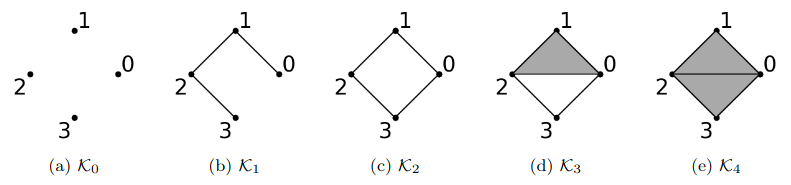
\includegraphics[width=\textwidth]{filtration}
        \centering
        \caption{Exemple de complexe simplicial, avec des simplexes de différentes dim et faces}
    \end{figure}
    
\end{frame}

\begin{frame}
    \frametitle{Définitions}
    \begin{block}{Filtration}
        Suite croissante pour l'inclusion de complexes simplicials
    \end{block}

    \begin{figure}
        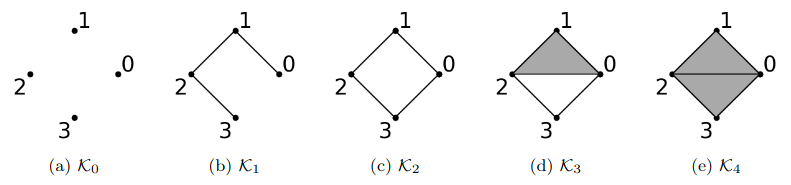
\includegraphics[width=\textwidth]{filtration}
        \centering
        \caption{Exemple de filtration}
    \end{figure}

    \begin{block}{Classe d'homologie}
        Intuitivement, elle représente un trou en dimension $n$

    \end{block}
\end{frame}

\begin{frame}
    \frametitle{Plan d'attaque}
    \itemize{
        \item Construire une filtration à partir d'un ensemble discret de points
        \item Application de l'algorithme \textit{standard}
        \item Récupération des classes d'homologies
    }

\end{frame}

\begin{frame}
    \frametitle{Théorème central}
\end{frame}

\begin{frame}
    \frametitle{Définition de la distance}
    
    \begin{block}{Distance}
        On définit la distance $d$ entre deux stations de metro $x$ et $y$ : 
        $$ d(x,y) = \frac{1}{2}(min(t_{pied}(x,y), t_{voiture}(x,y)) + min(t_{pied}(y,x), t_{voiture}(y,x)))$$
    \end{block}
\end{frame}

\begin{frame}
    \frametitle{Définition des complexes pondérés de Vietoris-Rips}
    
    
\end{frame}

\begin{frame}
    \frametitle{Lien entre les complexes et les stations de métros}
    
    
\end{frame}

\begin{frame}
    \frametitle{Récupération des données}
    Pour le calcul des temps de trajet :  apidocs.geoapify.com

    Pour la récupération des stations et des temps d'attentes moyens : transport.data.gouv.fr
\end{frame}

\begin{frame}
    \frametitle{Prératif de l'algorithme : Ordre total sur les simplexes}
\end{frame}


\begin{frame}
    \frametitle{Préparatif de l'algorithme : Matrice de brodure}
\end{frame}


\begin{frame}[fragile]
    \frametitle{Application de l'algorithme}
      \begin{lstlisting}
for j=1 to n do
    while il existe i < j avec Low(i) = j do
        Ajouter la colonne i a j
      \end{lstlisting}
  \end{frame}


\begin{frame}
    \frametitle{Compréhension du résultat en sortie}
\end{frame}

\begin{frame}
    \frametitle{Résultats et conclusion}

    \begin{figure}[h]
        \begin{minipage}[c]{.42\linewidth}
            \centering
            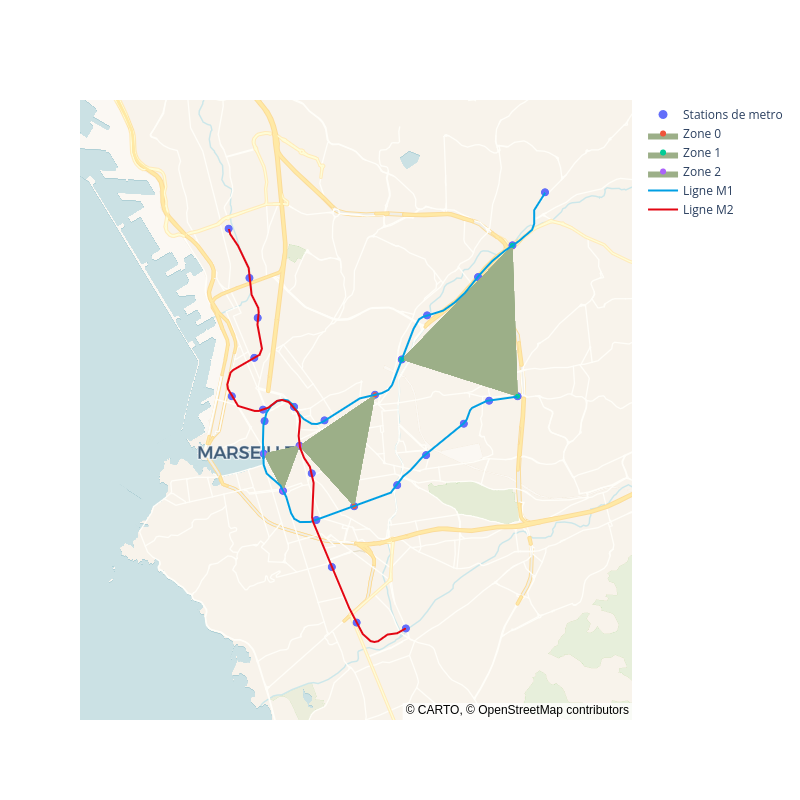
\includegraphics[width=1.1\textwidth]{../../Code/images/marseille.png}
            \caption{Marseille}
        \end{minipage}
        \hfill
        \begin{minipage}[c]{.42\linewidth}
            \centering
            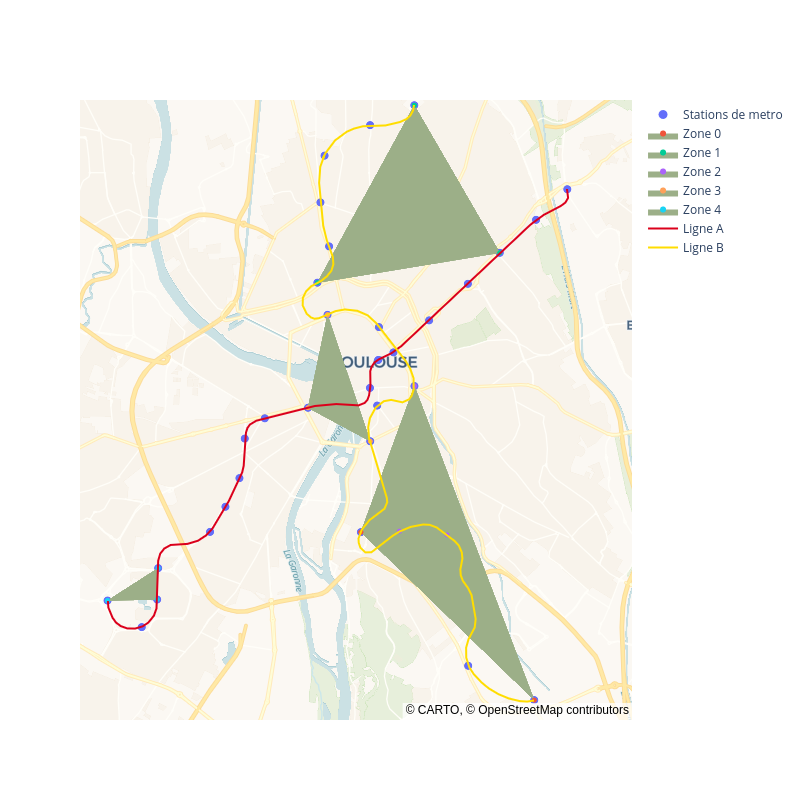
\includegraphics[width=1\textwidth]{../../Code/images/toulouse.png}
            \caption{Toulouse}
        \end{minipage}
    \end{figure}
\end{frame}

\begin{frame}
    \frametitle{Annexe}
    \begin{block}{Définition d'une variété}
        
    \end{block}
    \begin{block}{Définition d'un cycle}
        Un cycle est une sous-variété fermée.
    \end{block}
    \begin{block}{Définition d'une limite}
        Une limite est un cycle qui est également la limite d'une
        sous-variété 
    \end{block}
    \begin{block}{Définition d'une classe d'homologie}
        Une classe d'homologie est une classe d'équivalence de 
        cycles modulo une limite : elle est donc représentée par un
        cycle qui n'est la limite d'aucune sous-variété, il représente 
        donc un trou, une variété dont la limite serait ce cycle, mais qui n'est pas là
    \end{block}
\end{frame}

\begin{frame}
    \frametitle{Annexe : Diagrammes de persistance}
    % \begin{figure}
    %     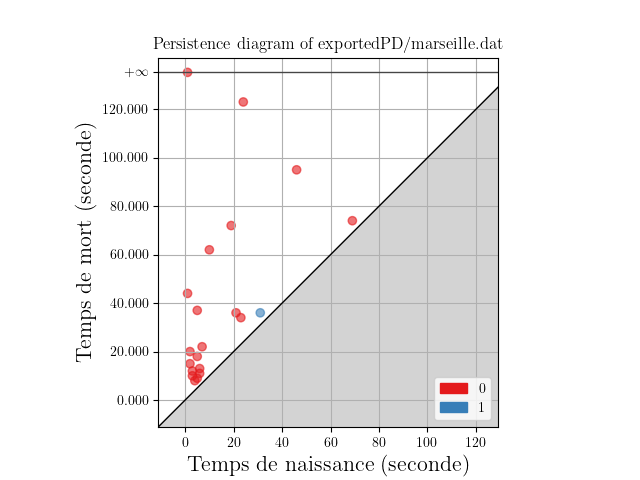
\includegraphics[width=0.7\textwidth]{pd_marseille}
    %     \centering
    %     \caption{Diagramme de persistance}
    % \end{figure}

    \begin{figure}[h]
        \begin{minipage}[c]{.45\linewidth}
            \centering
            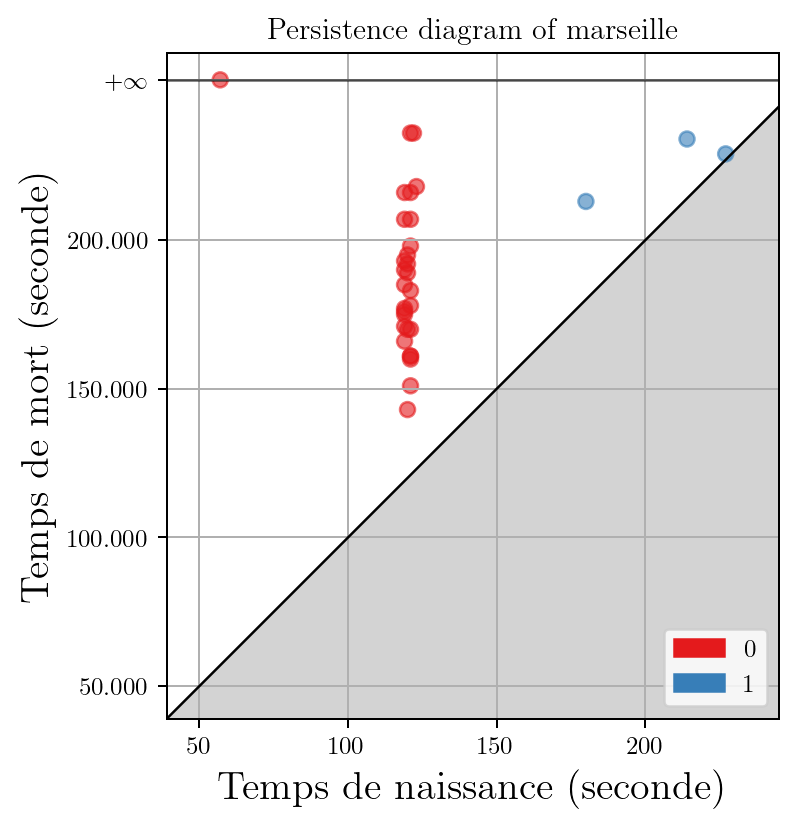
\includegraphics[width=1\textwidth]{../../Code/images/pd_marseille.png}
            \caption{Diagramme de persistance de Marseille}
        \end{minipage}
        \hfill
        \begin{minipage}[c]{.45\linewidth}
            \centering
            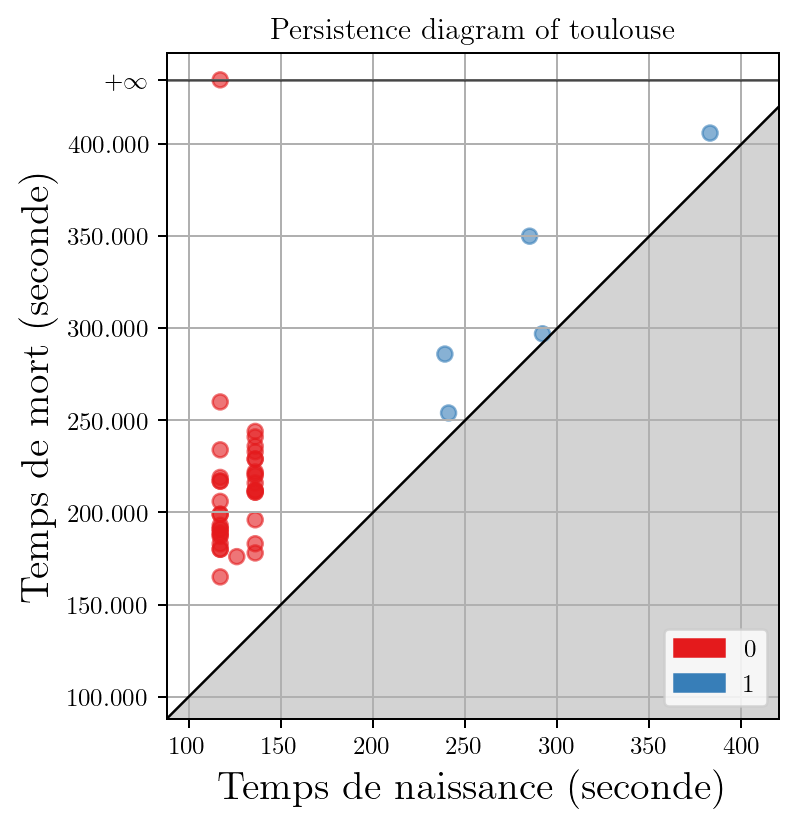
\includegraphics[width=1\textwidth]{../../Code/images/pd_toulouse.png}
            \caption{Diagramme de persistance de Toulouse}
        \end{minipage}
    \end{figure}
\end{frame}


\end{document}